\documentclass[11pt,a4paper]{article}

% Define page geometry
\usepackage{geometry} \geometry{left=2.2cm, right=2.2cm, top=2.2cm, bottom=2cm}
\parskip 0.15cm 
\setlength{\parindent}{0cm} 
\usepackage{pdflscape}
\usepackage[document]{ragged2e}

% Text formatting
\usepackage[T1]{fontenc}  % Set font

\usepackage{lineno}  % Line numbers

\usepackage{amssymb}  % Symbols
\usepackage{textcomp}
\newcommand{\textapprox}{\raisebox{0.5ex}{\texttildelow}}  % Command for a good tilde

\linespread{1.5}  % Linespacing

\usepackage{xcolor} \newcommand{\todo}[1]{\textcolor{red}{\textbf{#1}}}   %

\usepackage{lineno}

% Tables
\usepackage{multirow} \setlength{\tabcolsep}{4pt}

% Image handling
\usepackage{graphicx} 

\makeatletter \g@addto@macro\@floatboxreset\centering  
\makeatother

\graphicspath{ {img/} }  % Define image path

\usepackage{subfig}  % Compound figures

\usepackage{float}  % Precise figure location

% Bibliography management
\usepackage[style=authoryear, natbib=true, backend=biber]{biblatex}
\addbibresource{lidar.bib}

% Links within document, nice figure formatting
\usepackage[breaklinks]{hyperref} \definecolor{links}{RGB}{0,0,0} \hypersetup{
	breaklinks, colorlinks=true, linkcolor=links, anchorcolor=links,
	citecolor=links, filecolor=links, menucolor=links, runcolor=links,
	urlcolor=links, pdfauthor={John L. Godlee} }
	\def\subsectionautorefname{section} \def\subsubsectionautorefname{section}

\newcommand{\beginsupplement}{% 
	\setcounter{table}{0}
	\renewcommand{\thetable}{S\arabic{table}}% 
	\setcounter{figure}{0}
	\renewcommand{\thefigure}{S\arabic{figure}}% 
}
     
% Variables
\newcommand{\rawpt}{2.9e+08}
\newcommand{\voxelpt}{4.5e+07}
\newcommand{\subpt}{2.1e+07}


\newcommand{\titletext}{Species diversity and stand structure as drivers of canopy complexity in southern African woodlands}

\begin{document}

{\LARGE{\titletext{}}}

\linenumbers

\section*{Abstract}

\section{Introduction}

Canopy structure describes the spatial distribution and density of canopy foliage, comprising the primary interface between trees, the atmosphere and sunlight. Canopy structural complexity, i.e. the spatial heterogeneity of foliage distribution through the canopy, has been positively linked to canopy productivity \citep{Hardiman2011,Chen2012,Law2001,Baldocchi2001,Morin2015}. The characterisation of tree canopy structure in wooded ecosystems constitutes a long-standing field of research that has been fundamental to interpreting, modelling, and improving understanding of ecosystem function \citep{Watt1947, Whittaker1969, Horn1971, Maarel1996}. It is therefore essential to understand the drivers of variation in canopy structural complexity to improve modelling of earth-atmosphere carbon fluxes.

At continental scales, variation in canopy height and canopy cover, two coarse measures of canopy structure both of which have been shown to affect woody productivity and correlate with woody biomass \citep{}, can largely be explained by climate and edaphic data \citep{GEDI}. Increased resource availability allows for larger trees and greater canopy closure \citep{}. At the scale of a single tree community however, where variation in climate and soil may be negligible, variation in canopy structure is thought to be affected principally by an interacting combination of tree canopy species composition \citep{}, and disturbance history through its effect on stand physical structure \citep{}. However, empirical testing of these mechanisms thought to drive canopy structure in natural wooded ecosystems remains sparse across many biomes \citep{}.

Following established biodiversity-ecosystem function theory, the niche partitioning of canopy space, i.e. the spatial complementarity of individual tree canopies, is thought to be a key mechanism underlying positive biodiversity-productivity effects in wooded ecosystems \citep{Pretzsch2014, Barry2019}. Biodiversity-ecosystem function theory predicts that crown complementarity and thus canopy complexity and foliage density should increase with tree diversity in the local neighbourhood, increasing standing biomass and woody productivity, as coexisting species must occupy non-identical niche space to avoid competitive exclusion \citep{}.

As well as the species diversity of trees in a local neighbourhood, the spatial distribution and relative size of those trees, i.e. stand structure, is also expected to affect canopy structural complexity. Heterogeneity in tree size, whether a result of species diversity, disturbance history or some other factor, is expected to increase crown complexity and overall canopy density as individuals of different sizes occupy different parts of the vertical canopy space \citep{}. Additionally, clustering of individuals in space is expected to increase canopy structural heterogeneity across a stand, but ultimately decrease total foliage density due to an increase in competitive interactions \citep{}. Clustering may occur as a result of disturbance history, or as a result of strong facilitation effects among individuals in a hostile environment \citep{Ratcliffe2017}.

The direction of relationships between species diversity, stand structure, and canopy complexity is unclear. While biodiversity-ecosystem function theory presents a species diversity-centric view, whereby diversity affects stand structure and canopy structure, it is possible that aspects of stand structure may influence observed species diversity through sampling effects. Woodlands with greater stem density are likely to have greater species diversity, for example, simply because there are more stems which could potentially constitute different species \citep{}. It is important therefore to account for variation in stem density within models predicting the effects of structural and species diversity on canopy structure, and to design measures of structural diversity that are not conflated with stem density.

While much work in the field of forest management has been done to test biotic drivers of tree canopy structure in temperate \citep{} and boreal forests \citep{}, mostly to inform commercial forestry management, similar work in the tropics is comparatively scarce \citep{}. In dry tropical woodlands and savannas especially, tree canopy structure and its effect on ecosystem productivity has received little attention, possibly due to the misplaced assumption that woody productivity in these ecosystems does not represent a globally significant carbon flux \citep{}, or that tree canopies in these smaller stature woodlands do not interact and compete for resources to the same degree as in large stature forests \citep{}. In recent years however, it has been shown that dry tropical woodlands represent the largest uncertainty in our estimates of the terrestrial carbon cycle \citep{Quere2018, Ahlstrom2015}. \citet{Sitch2015} demonstrated the dominant role of the dry tropics in driving variability in the terrestrial carbon sink, and showed that the dry tropics are the fastest increasing component of the terrestrial carbon sink. Part of this uncertainty arises from our lacking a nuanced understanding of how species composition and structure affect ecosystem function in these ecosystems, which conceptually underpins the Dynamic Global Vegetation Models (DGVMs) fed into global carbon dynamics models. The pertinence of this knowledge gap has prompted further research of the biotic drivers of variation in productivity in the dry tropics, and momentum in this field of research is building, to create general theories of the ecosystem function of the dry tropics \citep{}.

Canopy structure is multi-dimensional and has previously been explained using a plethora of simple metrics that originated in forest and community ecology \citep{}. Assessments of canopy structure in the dry tropical have most often modelled tree canopies as a series of ellipses (2D) or ellipsoids (3D) based on field measurements with measuring tapes \citep{}. Measurements of this kind are time consuming and yet are an over-simplification of canopy structure \citep{}. Alternatively, canopy cover is often measured using indirect optical methods which partition sky from canopy material, i.e. with hemispherical photography or the commonly used LAI-2000, providing a 2D representation of the canopy but lacking information on vertical canopy structure. In recent years, particularly in temperate and boreal forests, LiDAR (Light Detection And Ranging) has emerged as a suitable technology for rapidly and precisely assessing canopy structure in 3D, conserving information on 3D structure of the calibre that is required to understand it's complexities \citep{}.

In this study we applied terrestrial LiDAR techniques to woodland-savanna mosaics at two sites in southern Africa, with the aim of increasing our understanding of how various metrics of tree canopy structural complexity are affected by tree neighbourhood diversity and stand structure. Our overarching contention is that neighbourhoods of greater tree diversity and greater structural diversity allow greater canopy complexity and foliage density, resulting in higher productivity, and ultimately a more `forest-like' community, rather than an open canopy savanna.

\section{Materials and methods}

\subsection{Study sites}

Measurements were conducted at two sites, the first in Bicuar National Park, southwest Angola (S15.1$^\circ$, E14.8$^\circ$), and the second in and around Mtarure Forest Reserve, southeast Tanzania (S9.0$^\circ$, E39.0$^\circ$) (\autoref{map}). At each site, 1 ha (100x100 m) plots were sited in areas of miombo woodland vegetation, across a gradient of stem density. In Angola, 15 plots were sampled, while in Tanzania, seven were sampled following the curtailment of fieldwork due to COVID-19 travel restrictions. Fieldwork was conducted between February and April at both sites, during the peak growth period of each site in order to capture the highest foliage volume in the canopy.

\begin{figure}[H]
\centering
	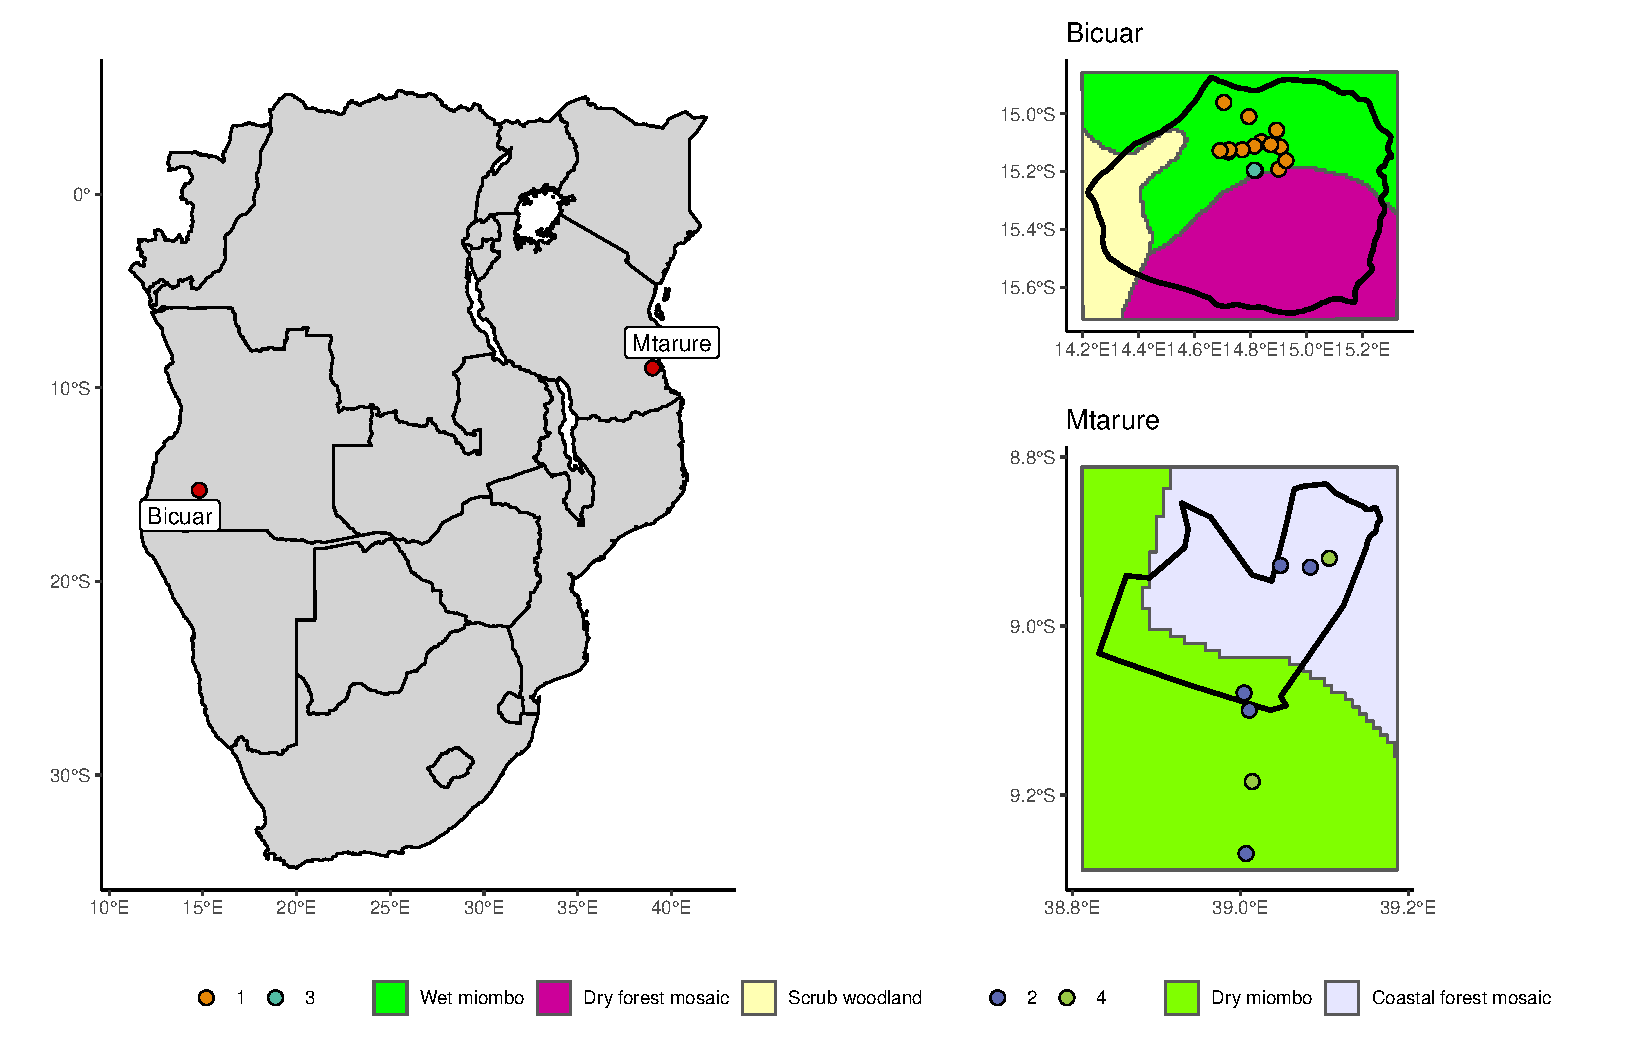
\includegraphics[width=\textwidth]{map}
	\caption{Location of study sites within southern Africa (a), and of 1 ha plots within each site. The blue polygons denote the boundaries of protected areas which encompass the majority of study sites, Bicuar National Park in Angola (b), and Mtarure Forest Reserve in Tanzania (c). The background of each site map is a re-classified version of the GlobCover global land cover classification \citep{Globcover}.}
	\label{map}
\end{figure}

\subsection{Field measurements}

Within each 1 ha plot we identified each stem >5 cm stem diameter to species, measured stem diameter (diameter at breast height - 1.3 m) and recorded stem location within the plot using tap measures. Each 1 ha plot was further subdivided into nine 10 m diameter circular subplots arranged in a regular grid, with a 15 m buffer from the plot edge and 35 m between subplots. For each subplot, we identified woody stems >5 cm diameter with canopy material inside the subplot. We measured the distance and direction from the subplot centre to each of these stems, as well as their projected crown area as an ellipse of two perpendicular crown diameter measurements.

Within each subplot, a variable number of scans were recorded using a Leica HDS6100 phase-shift Terrestrial Laser Scanner (TLS) \citep{Leica}. The number and position of scans within a subplot was determined by the arrangement of canopy material in the subplot. Scan positions were arranged to minimise shadows within the canopy of the subplot, and to maximise canopy penetration. The number of scans per subplot ranged between one and five in both sites. 

\subsection{Data analysis}

\subsubsection{Scan processing}

Point clouds from scans in each subplot were registered and unified using Leica Cyclone (version 9.1) \citep{Cyclone}, using five reflective targets visible to all scans. Point clouds were voxelised to cubic voxel sizes of different sizes depending on the application of the data. For subplot height profile estimation and gap fraction we used 5 cm\textsuperscript{3} voxels, and for whole plot canopy rugosity we used 10 cm\textsuperscript{3} voxels. Voxels were classed as filled if they intersected with one or more points. Variation in voxel size reflects the spatial scale of each analysis, and is bounded by the beam divergence of the scanner over longer distances \citep{}. Choosing voxels that are too small can result in pock-marked representations of surfaces that are especially problematic when calculating larger scale canopy structure metrics, such as canopy top roughness, while voxels that are too large can result in an over-estimation of plant volume when estimating canopy foliage density at the subplot scale \citep{Seidel2012, Cifuentes2014}. We used a noise reduction algorithm from \citet{} to discard points based on mean nearest neighbour distances. This effectively removed `ghost points' produced by partial interceptions and also removed many erroneous returns caused by airborne dust particles, which was common at our study sites. Raw points clouds for each subplot had a mean of \textapprox{}\rawpt{} points, \textapprox{}\voxelpt{} points after voxelisation, and \textapprox{}\subpt{} points after noise reduction.

Ground points were classified using the Progressive Morphological Filter (PMF) from \citet{Zhang2003}. Point cloud height was reclassified height based on this revised ground layer by measuring the vertical distance between the nearest ground point and each point.

We used ray-tracing to calculate canopy cover at the subplot centre from multiple TLS scans. Hemispherical images were created using the POV-ray software \citep{}. Voxels were converted to matt black cubes filling the voxel volume, with a white sky box and no light source. A `camera' with a 180\textdegree{} fisheye lens was placed at the subplot centre within POV-Ray, at a height of 1.8 m pointing directly upwards. The images produced by POV-Ray were analysed using Hemiphot \citep{Steege} to estimate canopy cover as the proportion of pixels filled by canopy material.

We calculated a number of metrics to describe different aspects of canopy complexity within each subplot in addition to canopy cover. Canopy height was measured as the 99th percentile of height of canopy material within the subplot. Layer diversity was calculated using Shannon entropy on foliage density of 0.5 m height bins through the tree canopy. The uniformity of foliage distribution was calculated by fitting a linear model to the cumulative foliage density profile, then extracting the standard error on the slope estimate of this linear model. The height of peak foliage density was calculated by fitting a loess model to the foliage height profile and extracting the height at which foliage density peaked.  

At the plot level, canopy complexity was measured with six metrics. Of these, canopy top roughness was measured as the standard deviation of canopy height across the plot, and canopy rugosity was measured according to \citet{Hardiman2011}, as the standard deviation of vertical and horizontal foliage density within 0.5 m cubic bins.

\subsection{Stand structure}

For each subplot, we calculated an adapted version of the Hegyi index to estimate crowding, as an alternative to stem density that works better to describe stand structure at small spatial scales \citep{Hegyi1974}. 

To estimate subplot structural diversity we calculated the coefficient of variation of stem diameter as a measure of the heterogeneity of tree size in the neighbourhood, and the coefficient of variation of neighbourhood crown area as a measure of the heterogeneity of tree canopy size.

At the plot level, we estimated the regularity of species spatial distribution using the spatial mingling index \citep{Gadow2002}. We also measured the uniformity of whole plot stem distribution using the winkelmass, which measures the degree of clustering of stems \citep{Gadow2002}. Finally, we calculated plot level stem density to estimate crowding.

\subsection{Statistical analysis}

Linear mixed effects models tested the effects of tree species diversity and stand structural diversity on canopy complexity. Mixed models were used to account for the highly nested sampling design of subplots within plots and plots within sites. Two sets of models were conducted, the first at the subplot level with random effects for plot nested within site, and the second at the plot level with random effects for site only. Separate models were fitted for each canopy complexity metric, resulting in six models at the subplot level and five models at the plot level. We compared the AIC values and Akaike weights of all models for a particular canopy complexity metric to find the `best model', i.e. the model which minimised variance in the fitted values, with penalties for complex model structure \citep{Akaike}.

To explore variation in tree species composition among plots and sites, we conducted a Non-metric Multi-dimensional Scaling (NMDS) analysis using tree species abundance in each plot. We excluded species with only one individual across all plots.  

\section{Results}

\subsection{Vertical canopy complexity}

\begin{figure}[H]
\centering
	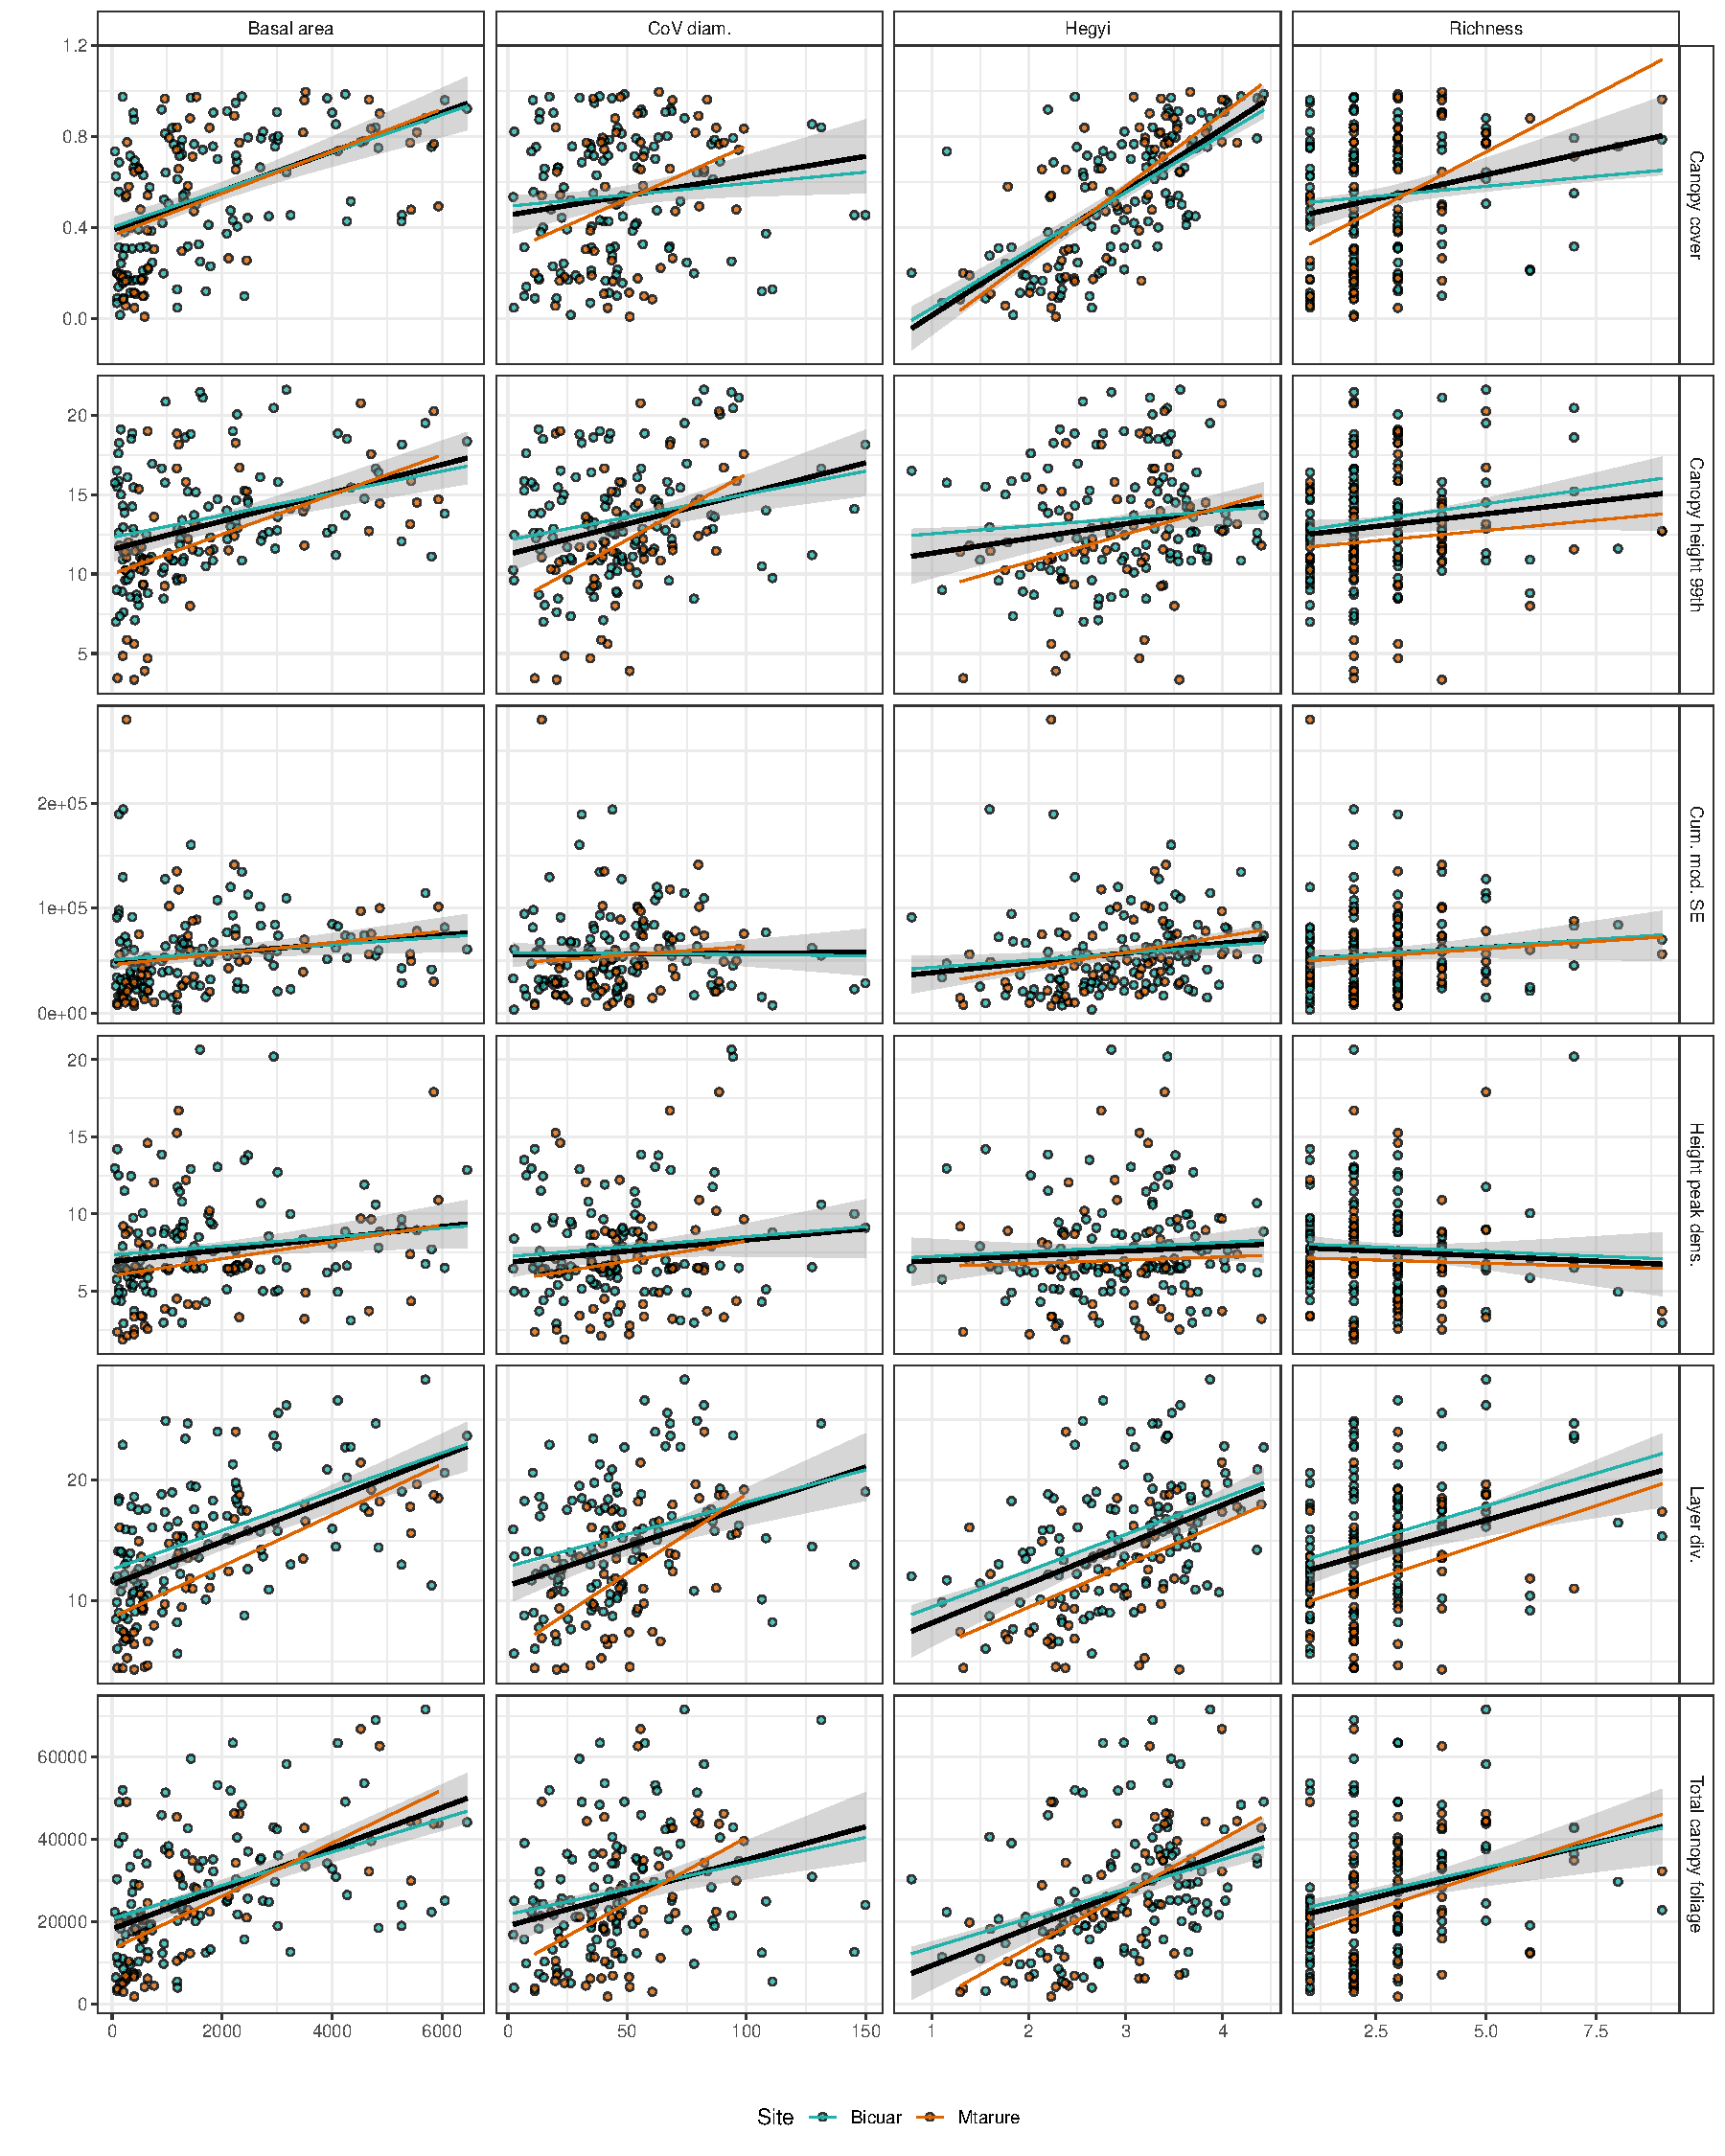
\includegraphics[width=0.8\textwidth]{subplot_canopy_bivar}
	\caption{Bivariate relationships between subplot canopy structure metrics (y axis) and diversity/stand structure metrics (x axis). Points and linear model lines of best fit are coloured by site. The black line of best fit is a linear model including both sites. See \todo{supp. material} for a comparison of linear model fits by site.}
	\label{subplot_canopy_bivar}
\end{figure}


Bivariate plots showed that subplot species diversity, measured by species richness of the tree neighbourhood around each 10 m diameter subplot, appeared to have weak but positive effects on canopy layer diversity and total canopy cover (\autoref{subplot_canopy_bivar}). The Hegyi crowding index and both stand structural diversity metrics had strong positive effects on canopy complexity, for all metrics except for uniformity of foliage distribution and height of peak foliage density. The two sites in our study had similar bivariate relationships, with interaction effects of site in the bivariate linear models being non-significant in all cases \todo{(supp. material)}.

Linear mixed effects models showed that species richness of the subplot neighbourhood had variable effects across different measures of canopy structure, but the effect sizes were not significant (slope standard errors not overlapping zero) for any model (\autoref{height_profile_mod_rich_slopes_sites}). One exception is the negative effect of richness on canopy height in Mtarure only. As in the bivariate plots, the Hegyi crowding index had strong positive effects on three of six canopy complexity metrics. Variation in stem diameter had a positive effect on layer diversity and total foliage density, and a marginally significant positive effect on canopy height. Variation in crown area did not have consistent effects on any canopy complexity metric.

\begin{figure}[H]
\centering
	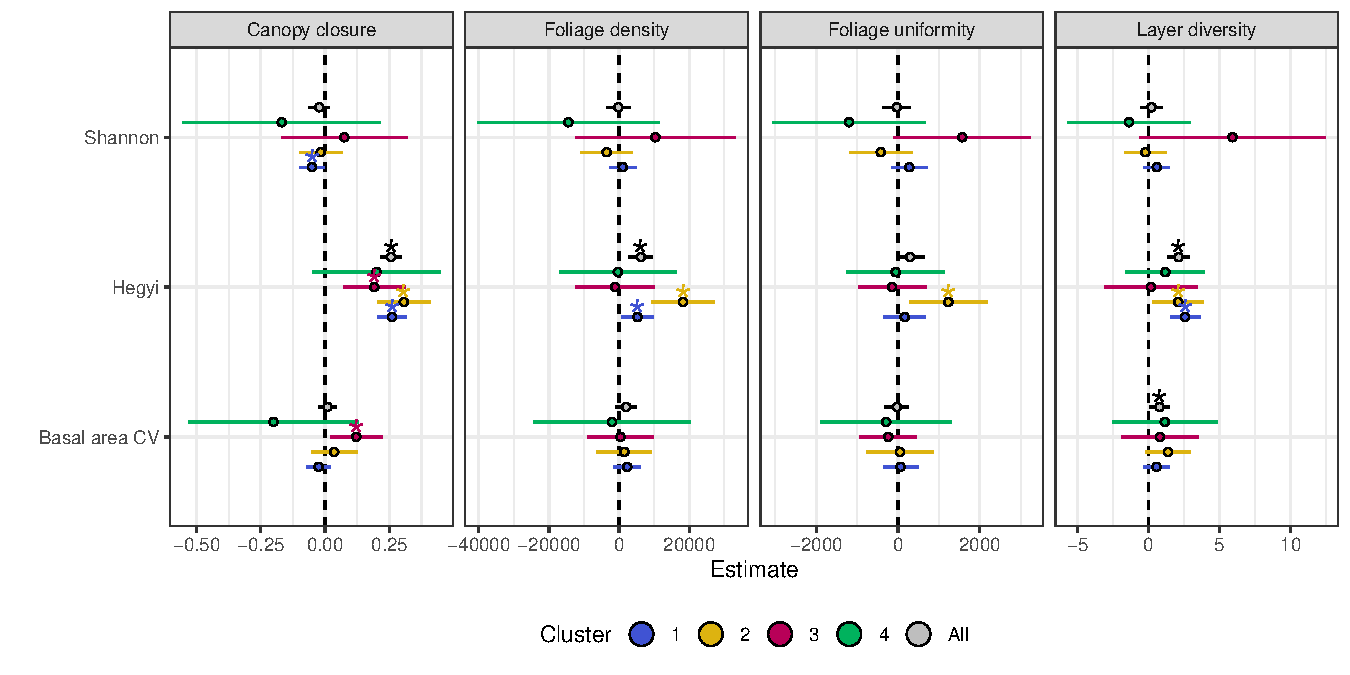
\includegraphics[width=\textwidth]{height_profile_mod_rich_slopes_sites}
	\caption{Standardized fixed effect slopes for each model of a canopy structure metric. Slope estimates are $\pm$1 standard error. Slope estimates where the interval (standard error) does not overlap zero are considered to be significant effects. Points are coloured according to site.}
	\label{height_profile_mod_rich_slopes_sites}
\end{figure}

The model selection process showed that the best model for layer diversity included species richness. Stand structural diversity metrics were included in the best models for all canopy complexity metrics except for canopy cover, which was predicted solely by the Hegyi crowding index. Models of layer diversity, total foliage density, and canopy cover were predicted well by a combination of crowding and stand structural diversity. Models of height of peak foliage density, canopy height, and uniformity of foliage distribution were poorly constrained by the fixed effects, with R\textsuperscript{2}\textsubscript{m} of \textapprox{}5\%. The majority of the total model effect on canopy height came from the random effects of site and plot identity.

% latex table generated in R 4.1.0 by xtable 1.8-4 package
% Wed Aug 11 17:43:51 2021
\begin{table}[]
\centering
\caption{Explanatory variables included in the best model for each canopy structure variable. $\Delta$AIC shows the difference in model AIC value compared to a null model which included only the hegyi crowding index and the random effects of vegetation type and plot. R\textsuperscript{2}\textsubscript{c} is the R\textsuperscript{2} of the best model, while R\textsuperscript{2}\textsubscript{m} is the R\textsuperscript{2} of the model fixed effects only.} 
\label{height_profile_sig_vars_dredge}
\begin{tabular}{lcccccc}
  \toprule
{Response} & {Hegyi} & {Richness} & {CoV basal area} & {$\Delta$AIC} & {R\textsuperscript{2}\textsubscript{c}} & {R\textsuperscript{2}\textsubscript{m}} \\ 
  \midrule
Layer diversity & \checkmark &  & \checkmark & 37.4 & 0.50 & 0.17 \\ 
  Foliage density & \checkmark &  & \checkmark & 77.7 & 0.28 & 0.19 \\ 
  Foliage uniformity & \checkmark &  &  & 37.4 & 0.12 & 0.05 \\ 
  Canopy closure & \checkmark &  &  & 104.0 & 0.63 & 0.49 \\ 
   \bottomrule
\end{tabular}
\end{table}



\subsection{Canopy rugosity}

Similar to the subplot analyses, at the whole-plot scale tree species diversity, measured here by the shannon index, tended to have weak positive effects on canopy complexity metrics, while stand structural diversity metrics had stronger positive effects (\autoref{canopy_rough_mod_bivar}). Strong positive relationships of basal area on canopy complexity are driven mostly by two plots with particularly low basal area in Mtarure, M3 and M4. These plots are sparse thorny savanna, dominated by \textit{Senegalia} spp. (\autoref{nmds}). Indeed, linear models using only plots in bicuar show divergent relationships. These two plots also have particularly low canopy cover, canopy height, and canopy top roughness, despite having similar tree species diversity and spatial distribution of trees (winkelmass) as other plots.

\begin{figure}[H]
\centering
	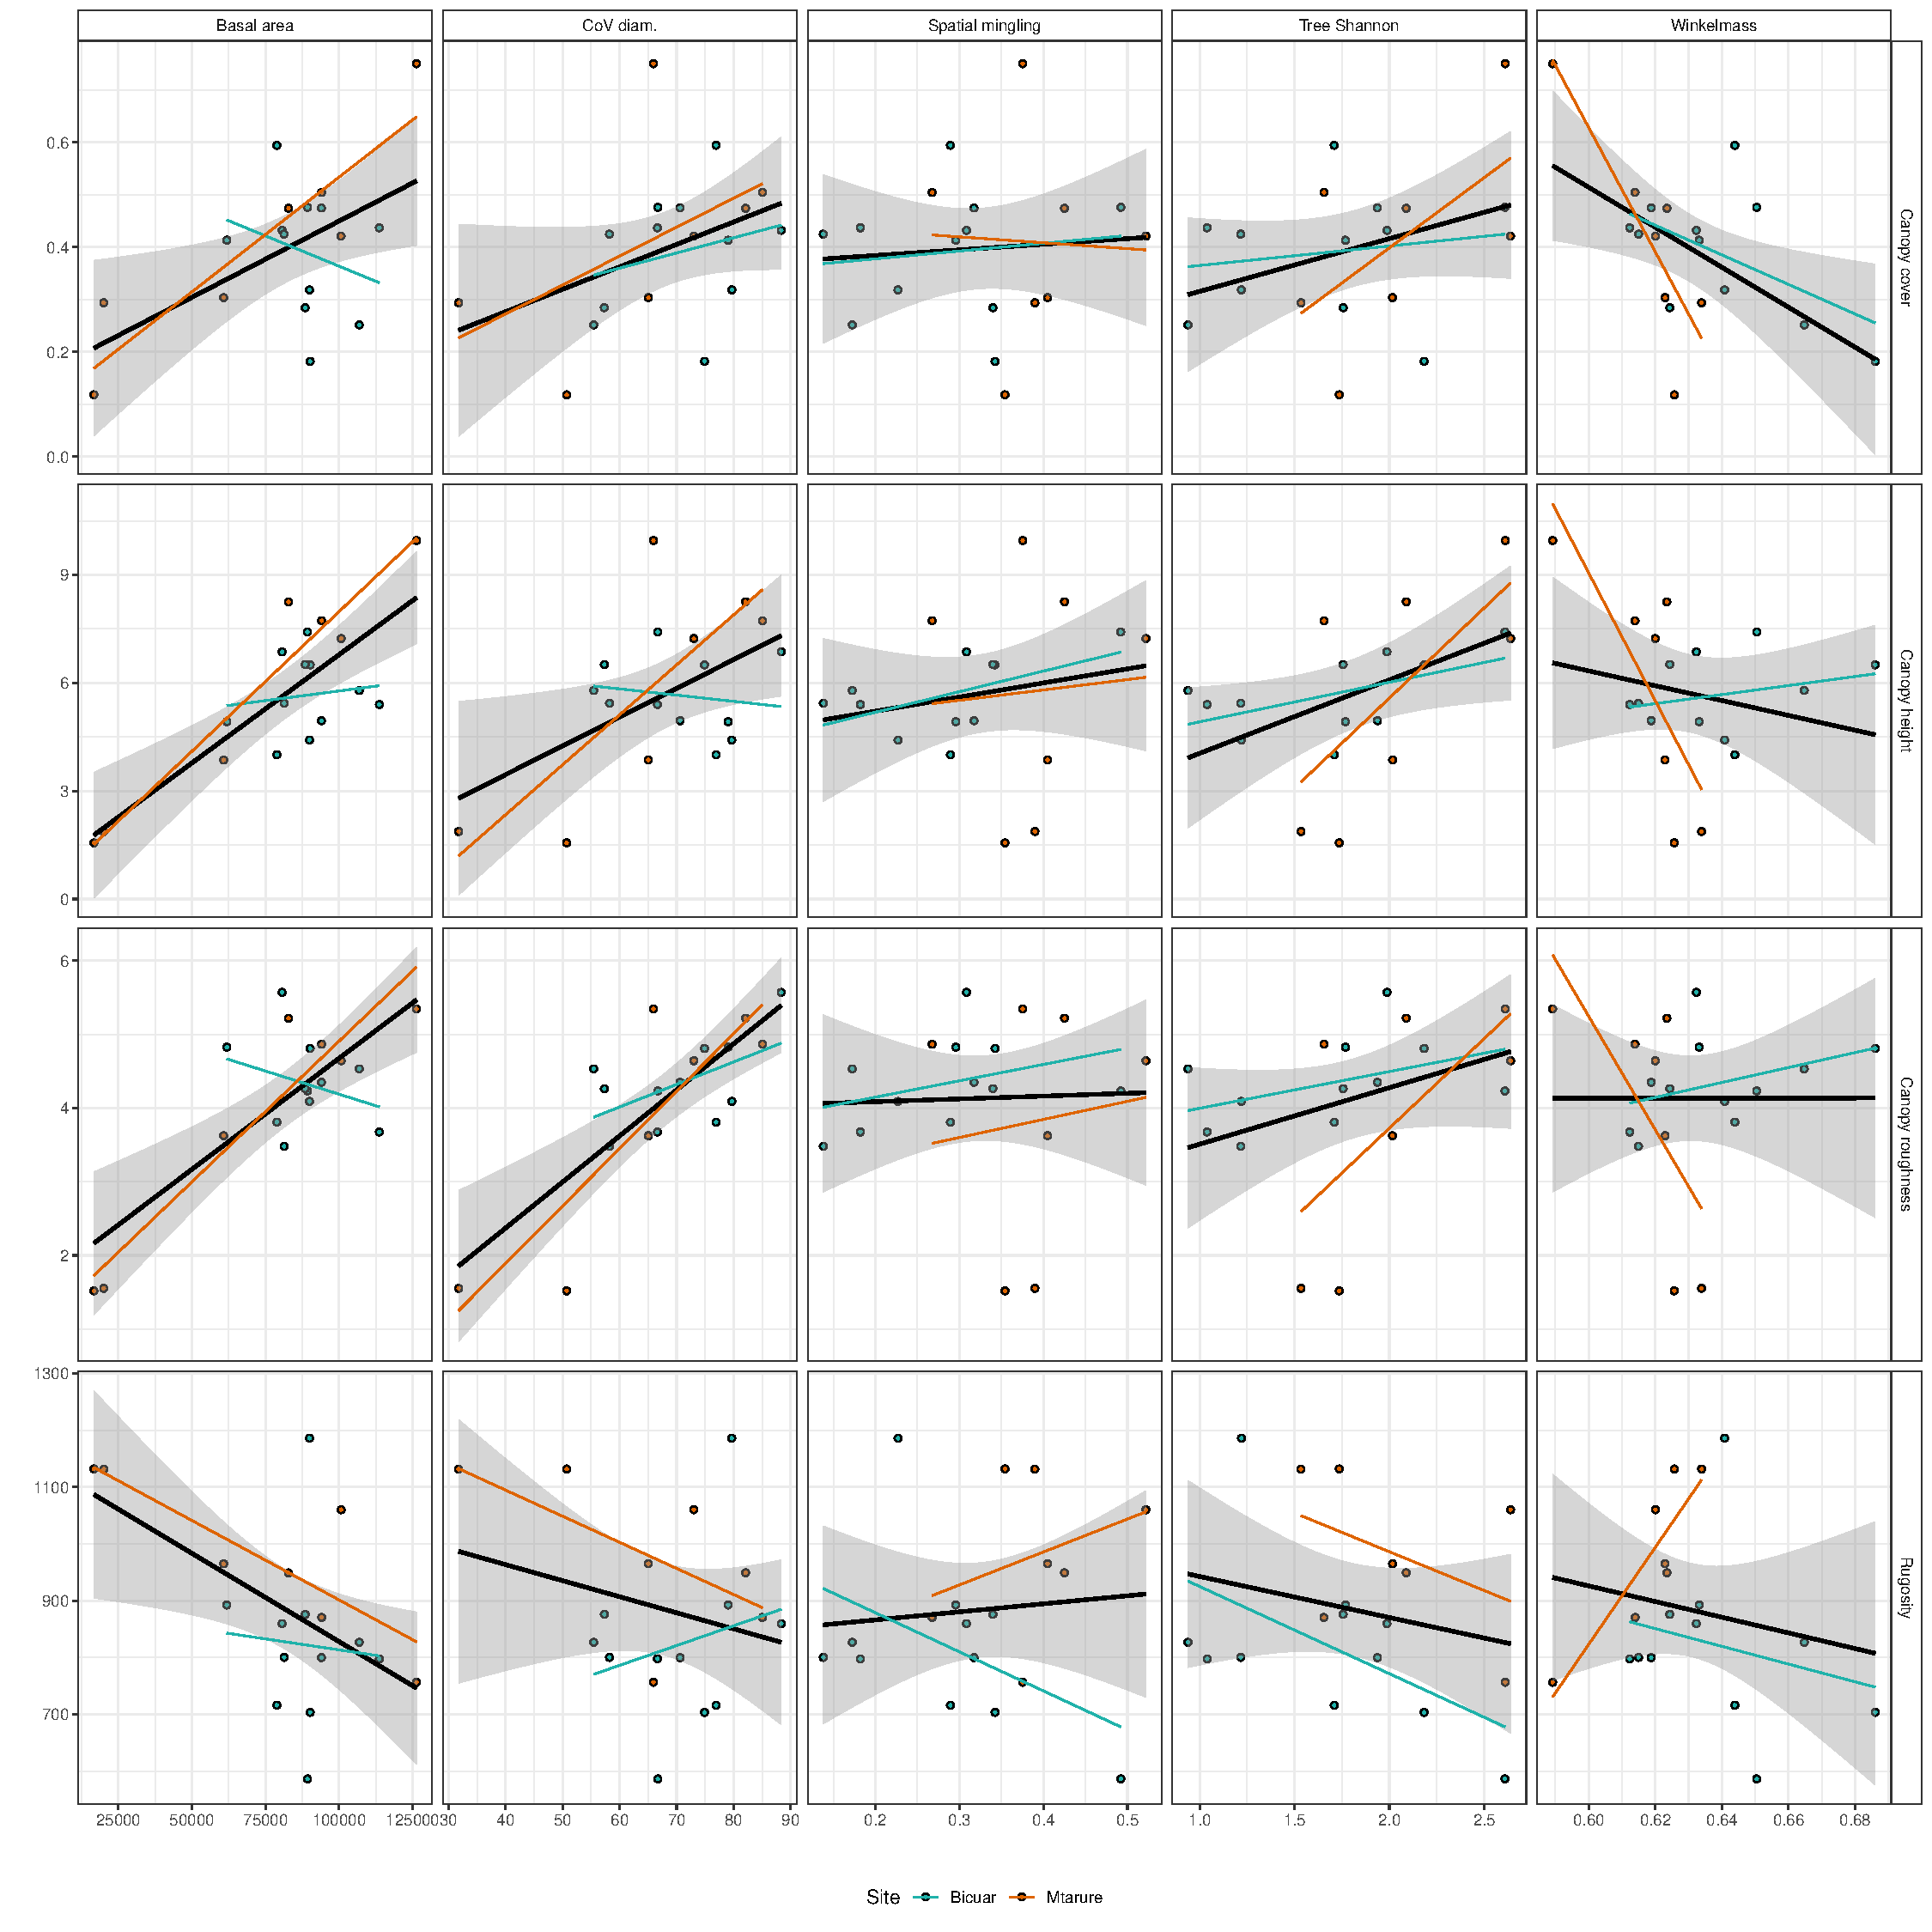
\includegraphics[width=\textwidth]{canopy_rough_mod_bivar}
	\caption{Bivariate relationships between diversiy and stand structure metrics (x axis) and whole-plot canopy structure metrics (y axis). Points and linear model lines of best fit are coloured by site. The thick black line of best fit is a linear model including both sites.}
	\label{canopy_rough_mod_bivar}
\end{figure}

Linear mixed effects models show that 

\begin{figure}[H]
\centering
	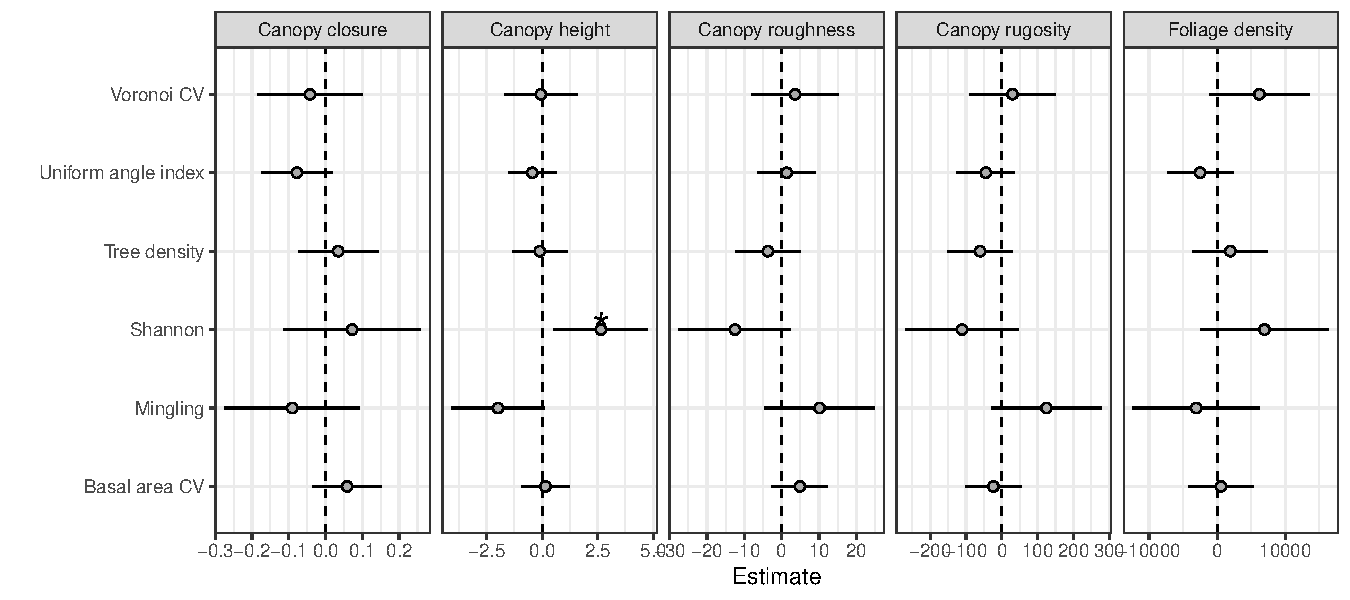
\includegraphics[width=\textwidth]{canopy_rough_slopes}
	\caption{Standardized fixed effect slopes for whole-plot canopy rugosity. Slope estimates are $\pm$1 standard error. Slope estimates where the interval (standard error) does not overlap zero are considered to be significant effects.}
	\label{canopy_rough_slopes}
\end{figure}

Model selection showed that all plot canopy complexity metrics except canopy rugosity were best modelled by a combination of basal area and either species diversity or structural diversity. 

% latex table generated in R 4.1.0 by xtable 1.8-4 package
% Mon Aug  9 15:44:59 2021
\begin{table}[H]
\centering
\begin{tabular}{rcccccccc}
  \hline
Response & Richness & Basal area & CoV basal area & Mingling & Winkelmass & $\Delta$AIC & R\textsuperscript{2}\textsubscript{c} & R\textsuperscript{2}\textsubscript{m} \\ 
  \hline
Canopy cover & \checkmark &  &  &  &  & -19.1 & 0.57 & 0.57 \\ 
  Canopy height & \checkmark & \checkmark &  &  &  & 9.0 & 0.77 & 0.77 \\ 
  Canopy roughness & \checkmark & \checkmark & \checkmark &  &  & 24.7 & 0.54 & 0.54 \\ 
  Rugosity &  & \checkmark &  &  &  & 43.7 & 0.57 & 0.35 \\ 
   \hline
\end{tabular}
\caption{Explanatory variables included in the best model for each plot-level canopy complexity metric. $\Delta$AIC shows the difference in model AIC value compared to a null model which included only the hegyi crowding index and the random effects of site and plot. R\textsuperscript{2}\textsubscript{c} is the R\textsuperscript{2} of the best model, while R\textsuperscript{2}\textsubscript{m} is the R\textsuperscript{2} of the model fixed effects only.} 
\label{canopy_sig_vars_dredge}
\end{table}



\begin{figure}[H]
\centering
	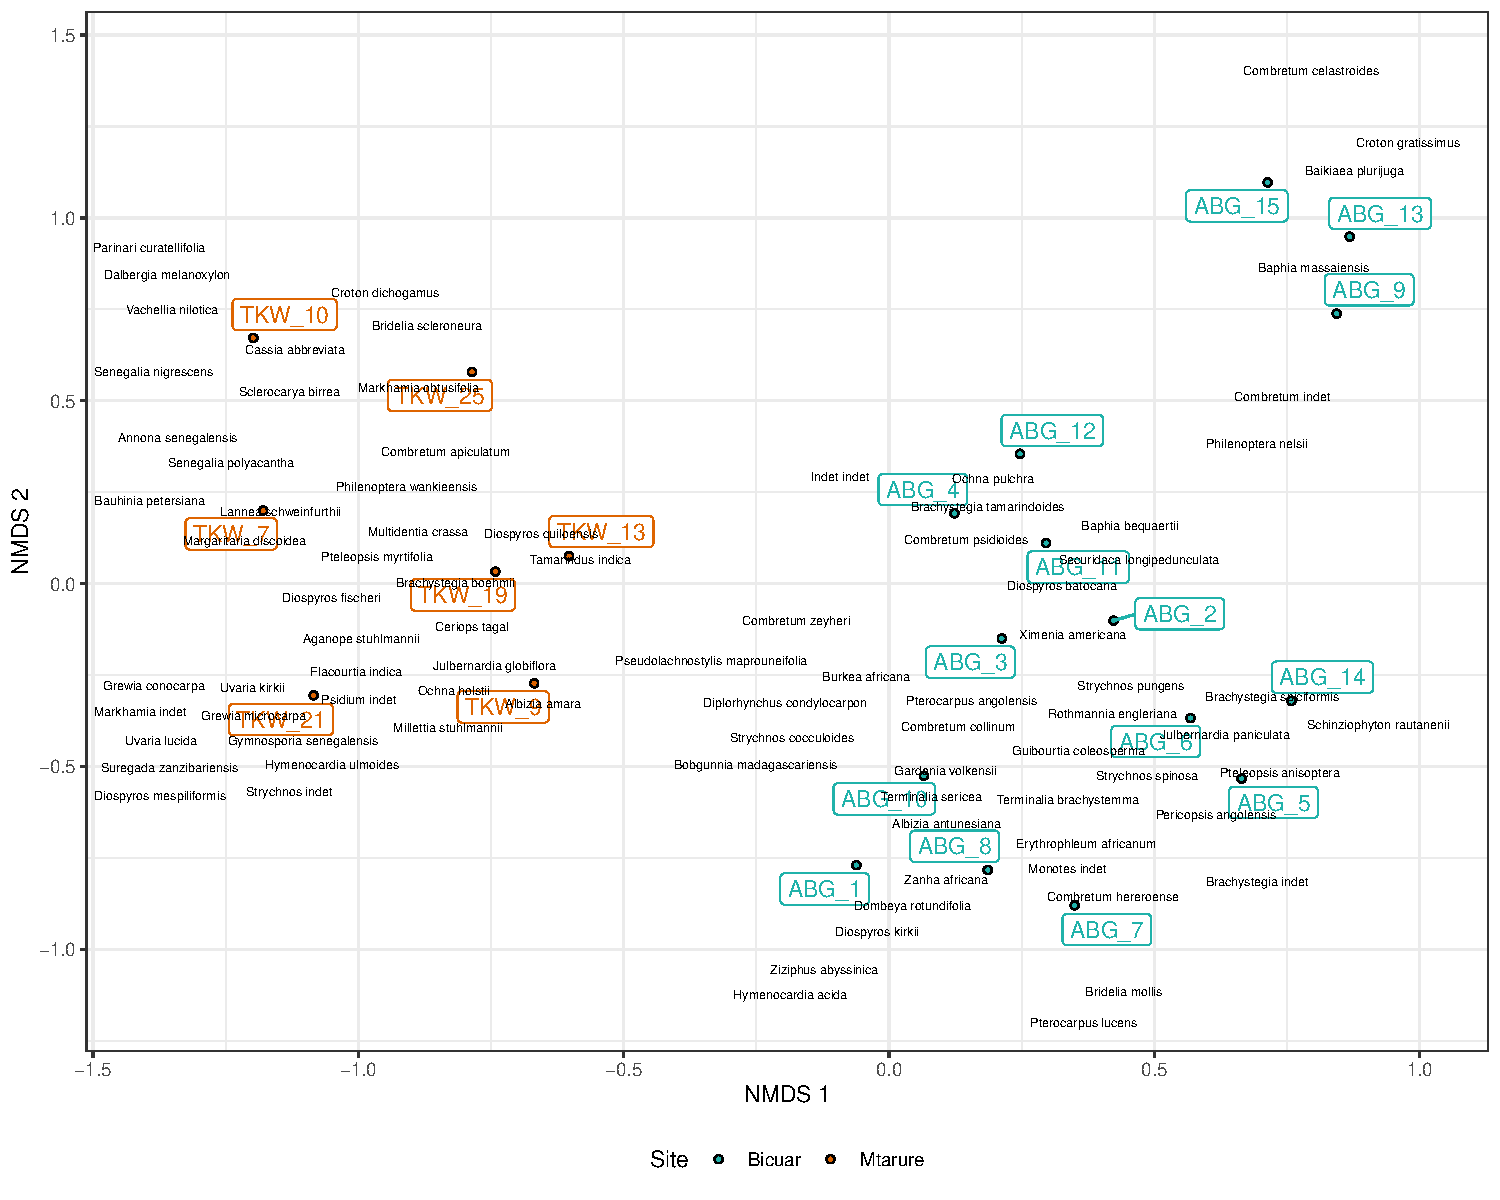
\includegraphics[width=\textwidth]{nmds}
	\caption{The first two axes of a Non-metric Multi-Dimensional Scaling (NMDS) analysis of tree species diversity in each plot. Species scores are labelled as black text, while plot scores are labelled as coloured points. Plots can be split into four principal groups: 1) B9, B13 and B15, dominated by \textit{Baikiaea plurijuga}; 2) the other Bicuar plots; 3) M2, M5, M6, and M7,dominated by \textit{Julbernardia} spp., \textit{Brachystegia} spp. and \textit{Ochna} spp.; 4) M1, M3, and M4, dominated by \textit{Senegalia} spp. and \textit{Vachellia} spp..}
	\label{nmds}
\end{figure}


\subsection{Comparing subplot and plot measures of canopy structure}

Plot-level and subplot-level canopy structure metrics were highly correlated in many cases (\autoref{canopy_rough_slopes}). Plot canopy height especially, tended to be strongly positively correlated with subplot canopy complexity. Additionally, as canopy top roughness increases, many subplot canopy complexity and density metrics increase. In the majority of cases, both sites had similar correlations of subplot and plot measures of canopy structure, with notable exceptions for plot roughness vs. layer diversity, plot roughnesss vs. canopy cover, and plot canopy height vs. canopy cover.

Variance of plot canopy height and plot roughness was larger in Mtarure than Bicuar. The increase in variance was caused by two particularly sparse thorny savanna plots in Mtarure, M3 and M4, which had very low canopy height and roughness.


\begin{figure}[H]
\centering
	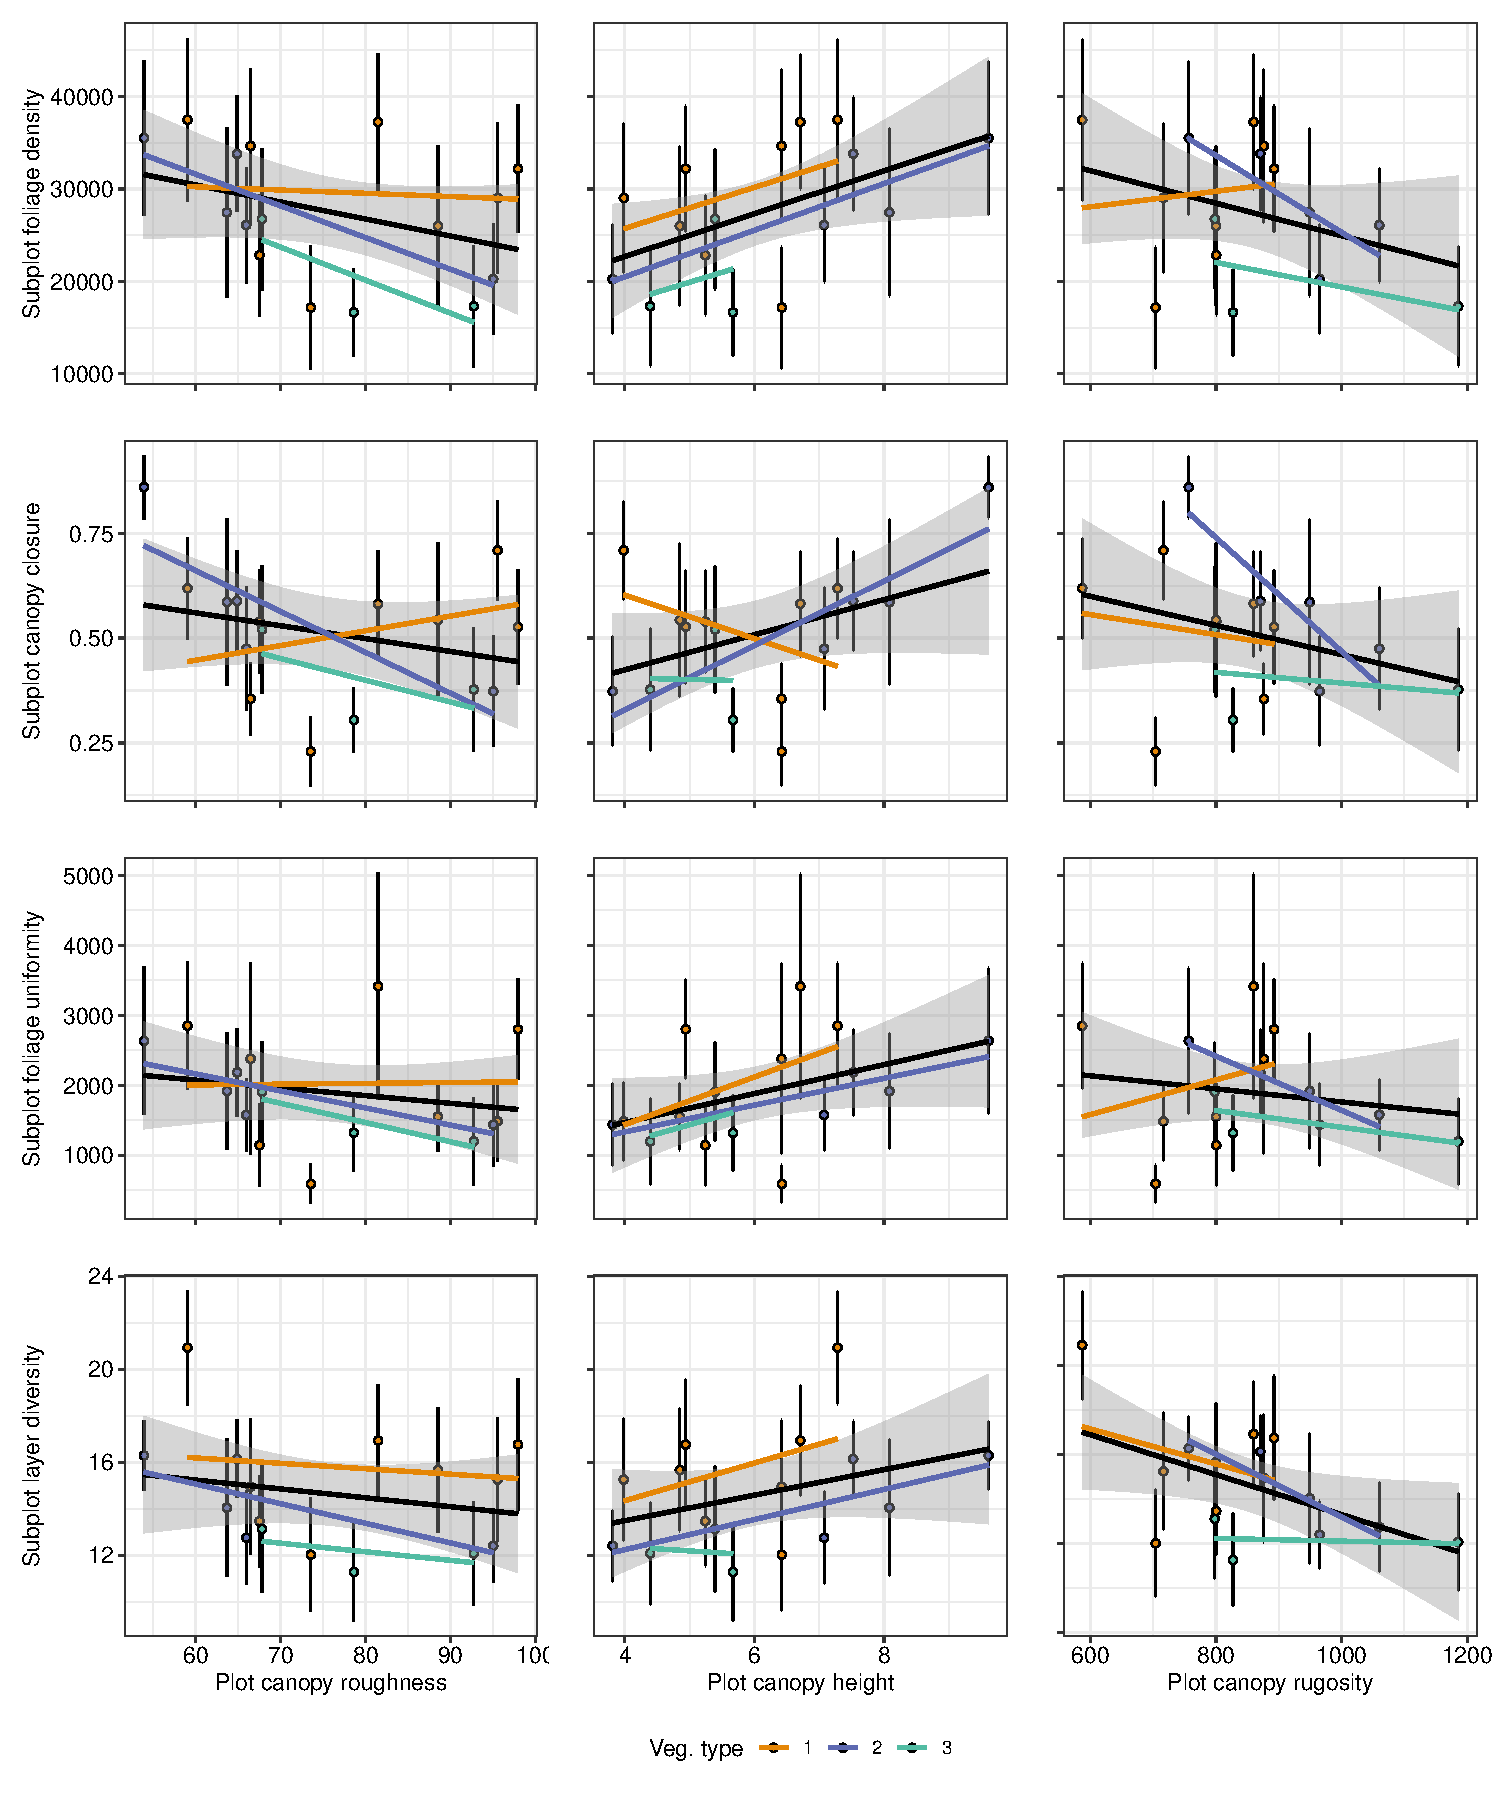
\includegraphics[width=\textwidth]{plot_subplot_bivar}
	\caption{Bivariate plots of canopy structural metrics at the subplot and plot-level. Each point represents the mean values of a single plot. Points and linear model fits are coloured according to site. The black linear model combines both sites. Error bars on points are the standard deviation of mean subplot metrics across the plot.}
	\label{plot_subplot_bivar}
\end{figure}



\section{Discussion}

We investigated the effects of tree species diversity and structural diversity on several metrics of canopy complexity that were hypothesised to affect plot productivity. Species diversity appeared to generally have weak positive effects on canopy complexity at both the subplot and plot scales, while stand structural diversity had much stronger effects. The strongest determinant of canopy complexity was stem crowding, as measured by basal area and the Hegyi crowding index.

The positive relationships between species richness and subplot canopy complexity metrics observed in the subplot bivariate models were not seen in the linear mixed effects models. This is likely because the observed species richness effect was itself driven by stand structure. The Hegyi crowding index increases with stem density, i.e. decreased distance of individuals from the subplot centre. Species richness also increases with stem density, as a greater number of individuals is more likely to hold more species simply through sampling effects. \citet{Jucker2015} however, did find that increased species diversity led to greater canopy packing in European forests, with trees in mixed forests having generally larger crowns. Our result that species diversity did not have consistent effects on canopy complexity may be specific to the vegetation type studied here. Southern African open woodlands are much more heavily affected by disturbance from fire and herbivory than temperate forests, meaning the effects of inter-specific competition are weakened as a driver of stand and canopy structure \citep{}.

Canopy structure at the plot level was less well predicted by stand structure and species diversity than subplot level canopy structure. Results at the plot level suggest that woodland vegetation type and basal area has the greatest effect on canopy complexity. The two thorny savanna plots in Mtarure produced strong positive effects of basal area and diameter variantion on canopy cover, canopy height, and canopy roughness, but when these plots are removed the remaining points do not produce strong relationships. 



\section{Conclusion}

\printbibliography

%\section{Supplementary Material} \beginsupplement

\end{document}
